\documentclass[twoside]{book}

% Packages required by doxygen
\usepackage{calc}
\usepackage{doxygen}
\usepackage{graphicx}
\usepackage[utf8]{inputenc}
\usepackage{makeidx}
\usepackage{multicol}
\usepackage{multirow}
\usepackage{textcomp}
\usepackage[table]{xcolor}

% Font selection
\usepackage[T1]{fontenc}
\usepackage{mathptmx}
\usepackage[scaled=.90]{helvet}
\usepackage{courier}
\usepackage{amssymb}
\usepackage{sectsty}
\renewcommand{\familydefault}{\sfdefault}
\allsectionsfont{%
  \fontseries{bc}\selectfont%
  \color{darkgray}%
}
\renewcommand{\DoxyLabelFont}{%
  \fontseries{bc}\selectfont%
  \color{darkgray}%
}

% Page & text layout
\usepackage{geometry}
\geometry{%
  a4paper,%
  top=2.5cm,%
  bottom=2.5cm,%
  left=2.5cm,%
  right=2.5cm%
}
\tolerance=750
\hfuzz=15pt
\hbadness=750
\setlength{\emergencystretch}{15pt}
\setlength{\parindent}{0cm}
\setlength{\parskip}{0.2cm}
\makeatletter
\renewcommand{\paragraph}{%
  \@startsection{paragraph}{4}{0ex}{-1.0ex}{1.0ex}{%
    \normalfont\normalsize\bfseries\SS@parafont%
  }%
}
\renewcommand{\subparagraph}{%
  \@startsection{subparagraph}{5}{0ex}{-1.0ex}{1.0ex}{%
    \normalfont\normalsize\bfseries\SS@subparafont%
  }%
}
\makeatother

% Headers & footers
\usepackage{fancyhdr}
\pagestyle{fancyplain}
\fancyhead[LE]{\fancyplain{}{\bfseries\thepage}}
\fancyhead[CE]{\fancyplain{}{}}
\fancyhead[RE]{\fancyplain{}{\bfseries\leftmark}}
\fancyhead[LO]{\fancyplain{}{\bfseries\rightmark}}
\fancyhead[CO]{\fancyplain{}{}}
\fancyhead[RO]{\fancyplain{}{\bfseries\thepage}}
\fancyfoot[LE]{\fancyplain{}{}}
\fancyfoot[CE]{\fancyplain{}{}}
\fancyfoot[RE]{\fancyplain{}{\bfseries\scriptsize Generated on Tue Nov 17 2015 11\-:43\-:05 for My Project by Doxygen }}
\fancyfoot[LO]{\fancyplain{}{\bfseries\scriptsize Generated on Tue Nov 17 2015 11\-:43\-:05 for My Project by Doxygen }}
\fancyfoot[CO]{\fancyplain{}{}}
\fancyfoot[RO]{\fancyplain{}{}}
\renewcommand{\footrulewidth}{0.4pt}
\renewcommand{\chaptermark}[1]{%
  \markboth{#1}{}%
}
\renewcommand{\sectionmark}[1]{%
  \markright{\thesection\ #1}%
}

% Indices & bibliography
\usepackage{natbib}
\usepackage[titles]{tocloft}
\setcounter{tocdepth}{3}
\setcounter{secnumdepth}{5}
\makeindex

% Hyperlinks (required, but should be loaded last)
\usepackage{ifpdf}
\ifpdf
  \usepackage[pdftex,pagebackref=true]{hyperref}
\else
  \usepackage[ps2pdf,pagebackref=true]{hyperref}
\fi
\hypersetup{%
  colorlinks=true,%
  linkcolor=blue,%
  citecolor=blue,%
  unicode%
}

% Custom commands
\newcommand{\clearemptydoublepage}{%
  \newpage{\pagestyle{empty}\cleardoublepage}%
}


%===== C O N T E N T S =====

\begin{document}

% Titlepage & ToC
\hypersetup{pageanchor=false}
\pagenumbering{roman}
\begin{titlepage}
\vspace*{7cm}
\begin{center}%
{\Large My Project }\\
\vspace*{1cm}
{\large Generated by Doxygen 1.8.6}\\
\vspace*{0.5cm}
{\small Tue Nov 17 2015 11:43:05}\\
\end{center}
\end{titlepage}
\clearemptydoublepage
\tableofcontents
\clearemptydoublepage
\pagenumbering{arabic}
\hypersetup{pageanchor=true}

%--- Begin generated contents ---
\chapter{R\-E\-A\-D\-M\-E}
\label{md_README}
\hypertarget{md_README}{}
S\-E\-N\-G 330, Assignment 2 
\chapter{Hierarchical Index}
\section{Class Hierarchy}
This inheritance list is sorted roughly, but not completely, alphabetically\-:\begin{DoxyCompactList}
\item \contentsline{section}{machine}{\pageref{classmachine}}{}
\begin{DoxyCompactList}
\item \contentsline{section}{bracelet}{\pageref{classbracelet}}{}
\item \contentsline{section}{elliptical}{\pageref{classelliptical}}{}
\item \contentsline{section}{lift}{\pageref{classlift}}{}
\end{DoxyCompactList}
\item \contentsline{section}{member}{\pageref{classmember}}{}
\begin{DoxyCompactList}
\item \contentsline{section}{bracelet}{\pageref{classbracelet}}{}
\end{DoxyCompactList}
\item Message\begin{DoxyCompactList}
\item \contentsline{section}{machines\-:\-:Machine}{\pageref{classmachines_1_1Machine}}{}
\item \contentsline{section}{machines\-:\-:Machines}{\pageref{classmachines_1_1Machines}}{}
\end{DoxyCompactList}
\item \contentsline{section}{machines\-:\-:Static\-Descriptor\-Initializer\-\_\-fitplanet\-\_\-2eproto}{\pageref{structmachines_1_1StaticDescriptorInitializer__fitplanet__2eproto}}{}
\end{DoxyCompactList}

\chapter{Class Index}
\section{Class List}
Here are the classes, structs, unions and interfaces with brief descriptions\-:\begin{DoxyCompactList}
\item\contentsline{section}{\hyperlink{classbracelet}{bracelet} }{\pageref{classbracelet}}{}
\item\contentsline{section}{\hyperlink{classelliptical}{elliptical} }{\pageref{classelliptical}}{}
\item\contentsline{section}{\hyperlink{classlift}{lift} }{\pageref{classlift}}{}
\item\contentsline{section}{\hyperlink{classmachines_1_1Machine}{machines\-::\-Machine} }{\pageref{classmachines_1_1Machine}}{}
\item\contentsline{section}{\hyperlink{classmachine}{machine} }{\pageref{classmachine}}{}
\item\contentsline{section}{\hyperlink{classmachines_1_1Machines}{machines\-::\-Machines} }{\pageref{classmachines_1_1Machines}}{}
\item\contentsline{section}{\hyperlink{classmember}{member} }{\pageref{classmember}}{}
\item\contentsline{section}{\hyperlink{structmachines_1_1StaticDescriptorInitializer__fitplanet__2eproto}{machines\-::\-Static\-Descriptor\-Initializer\-\_\-fitplanet\-\_\-2eproto} }{\pageref{structmachines_1_1StaticDescriptorInitializer__fitplanet__2eproto}}{}
\end{DoxyCompactList}

\chapter{Class Documentation}
\hypertarget{classbracelet}{\section{bracelet Class Reference}
\label{classbracelet}\index{bracelet@{bracelet}}
}
Inheritance diagram for bracelet\-:\begin{figure}[H]
\begin{center}
\leavevmode
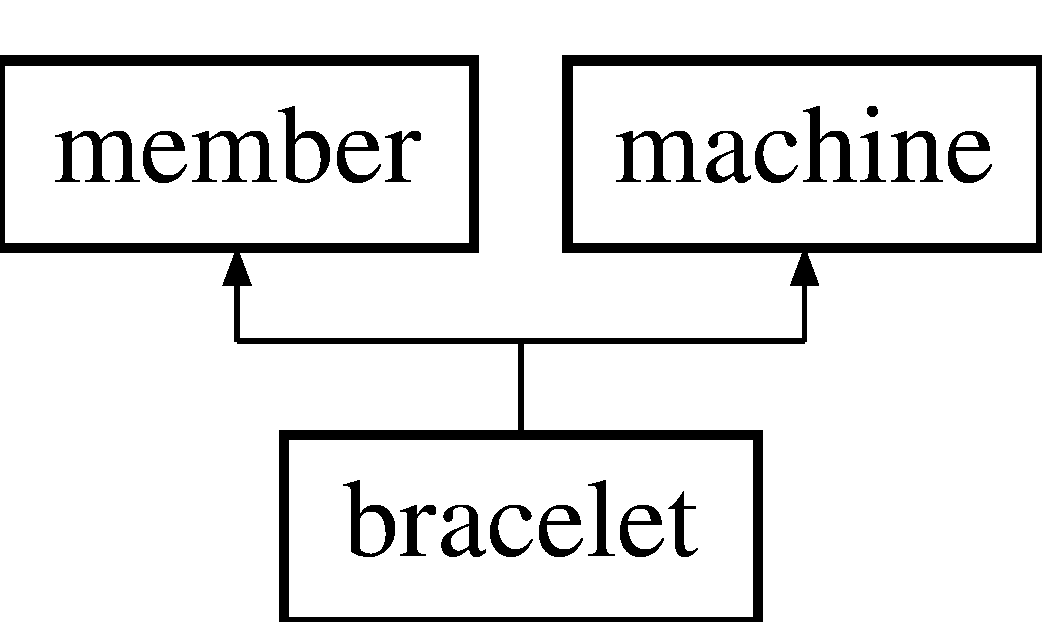
\includegraphics[height=2.000000cm]{classbracelet}
\end{center}
\end{figure}
\subsection*{Public Member Functions}
\begin{DoxyCompactItemize}
\item 
\hypertarget{classbracelet_a51b4e2907d3bd742bed3c5af8fb58e41}{{\bfseries bracelet} (char $\ast$)}\label{classbracelet_a51b4e2907d3bd742bed3c5af8fb58e41}

\item 
\hypertarget{classbracelet_a220850e5494aea041478ba50540ea58f}{char $\ast$ {\bfseries get\-\_\-owner} () const }\label{classbracelet_a220850e5494aea041478ba50540ea58f}

\item 
\hypertarget{classbracelet_a5df367d5e2c766f8070d892ed0735858}{std\-::vector$<$ \hyperlink{classmachine}{machine} $>$ {\bfseries machines\-\_\-used} () const }\label{classbracelet_a5df367d5e2c766f8070d892ed0735858}

\item 
\hypertarget{classbracelet_a7b27c0f1916a5a2ca1036e2f966ad431}{void {\bfseries change\-\_\-owner} (char $\ast$)}\label{classbracelet_a7b27c0f1916a5a2ca1036e2f966ad431}

\item 
\hypertarget{classbracelet_af335417478ad987d9df5521c430ac59d}{void {\bfseries remove\-\_\-owner} ()}\label{classbracelet_af335417478ad987d9df5521c430ac59d}

\item 
\hypertarget{classbracelet_a39485b59c215f4952da18b3bdb5aede0}{void {\bfseries add\-\_\-machine} (\hyperlink{classmachine}{machine})}\label{classbracelet_a39485b59c215f4952da18b3bdb5aede0}

\end{DoxyCompactItemize}


The documentation for this class was generated from the following files\-:\begin{DoxyCompactItemize}
\item 
bracelet.\-h\item 
bracelet.\-cpp\end{DoxyCompactItemize}

\hypertarget{classelliptical}{\section{elliptical Class Reference}
\label{classelliptical}\index{elliptical@{elliptical}}
}
Inheritance diagram for elliptical\-:\begin{figure}[H]
\begin{center}
\leavevmode
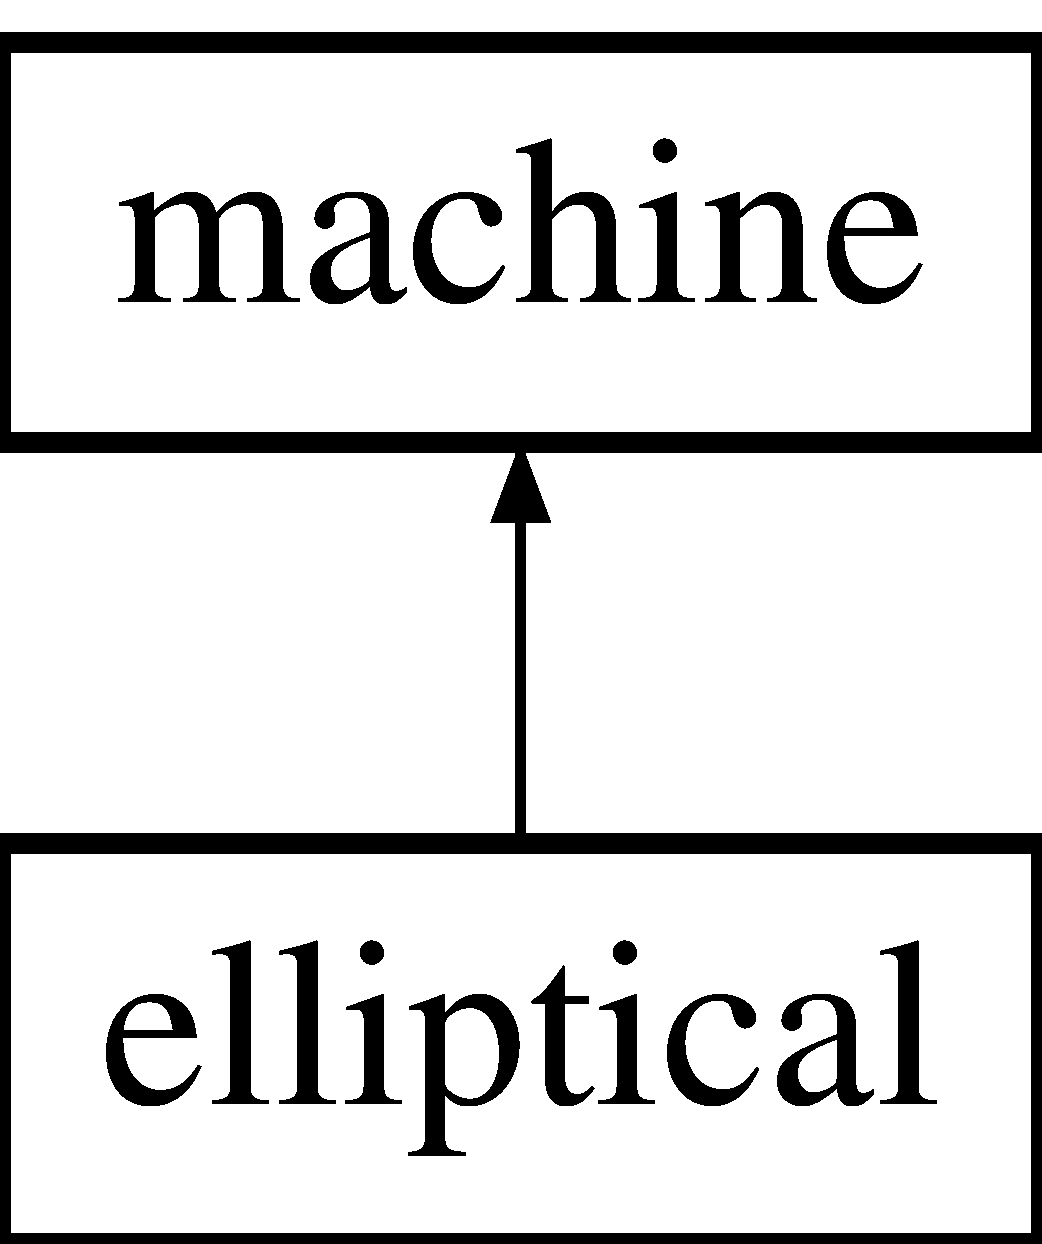
\includegraphics[height=2.000000cm]{classelliptical}
\end{center}
\end{figure}
\subsection*{Public Member Functions}
\begin{DoxyCompactItemize}
\item 
\hypertarget{classelliptical_a00cc443f8633d13f9b5a336b627d8cdf}{int {\bfseries time\-\_\-used} ()}\label{classelliptical_a00cc443f8633d13f9b5a336b627d8cdf}

\end{DoxyCompactItemize}


The documentation for this class was generated from the following files\-:\begin{DoxyCompactItemize}
\item 
elliptical.\-h\item 
elliptical.\-cpp\end{DoxyCompactItemize}

\hypertarget{classlift}{\section{lift Class Reference}
\label{classlift}\index{lift@{lift}}
}
Inheritance diagram for lift\-:\begin{figure}[H]
\begin{center}
\leavevmode
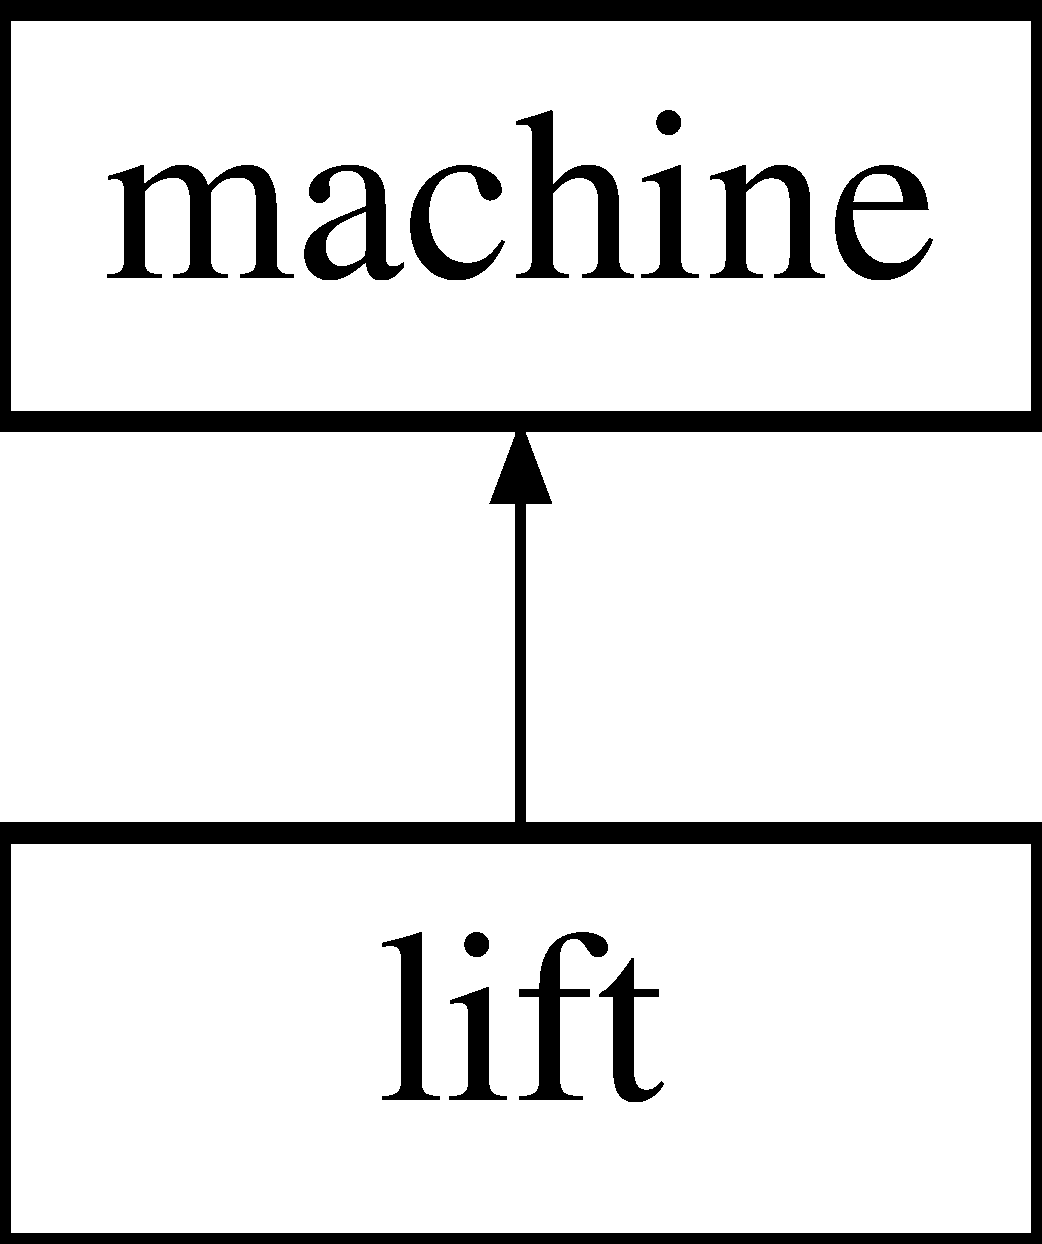
\includegraphics[height=2.000000cm]{classlift}
\end{center}
\end{figure}
\subsection*{Public Member Functions}
\begin{DoxyCompactItemize}
\item 
\hypertarget{classlift_a9f371f20603a92b21141ebc31503b0d7}{int {\bfseries repetitions} ()}\label{classlift_a9f371f20603a92b21141ebc31503b0d7}

\item 
\hypertarget{classlift_aaabecf780e0d0e1ed433fc92b301551f}{int {\bfseries weight\-\_\-lifted} ()}\label{classlift_aaabecf780e0d0e1ed433fc92b301551f}

\end{DoxyCompactItemize}


The documentation for this class was generated from the following files\-:\begin{DoxyCompactItemize}
\item 
lift.\-h\item 
lift.\-cpp\end{DoxyCompactItemize}

\hypertarget{classmachines_1_1Machine}{\section{machines\-:\-:Machine Class Reference}
\label{classmachines_1_1Machine}\index{machines\-::\-Machine@{machines\-::\-Machine}}
}
Inheritance diagram for machines\-:\-:Machine\-:\begin{figure}[H]
\begin{center}
\leavevmode
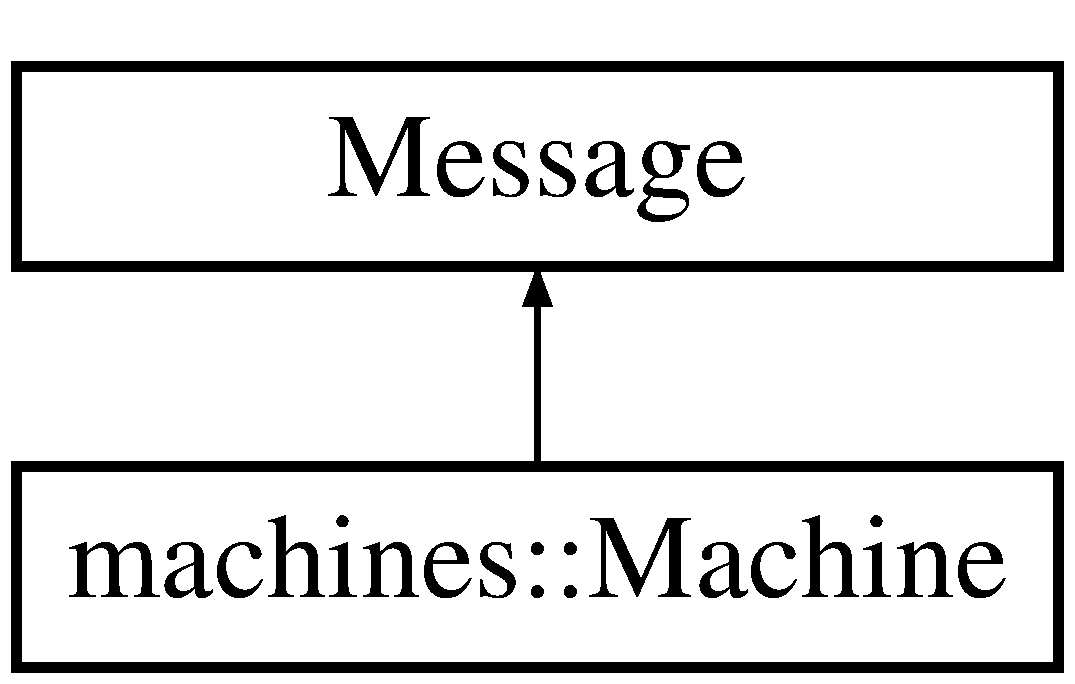
\includegraphics[height=2.000000cm]{classmachines_1_1Machine}
\end{center}
\end{figure}
\subsection*{Public Member Functions}
\begin{DoxyCompactItemize}
\item 
\hypertarget{classmachines_1_1Machine_a4bc25165182e6a979ef514463749076e}{{\bfseries Machine} (const \hyperlink{classmachines_1_1Machine}{Machine} \&from)}\label{classmachines_1_1Machine_a4bc25165182e6a979ef514463749076e}

\item 
\hypertarget{classmachines_1_1Machine_a446fbdac340914a6706dfe3251d7e9f7}{\hyperlink{classmachines_1_1Machine}{Machine} \& {\bfseries operator=} (const \hyperlink{classmachines_1_1Machine}{Machine} \&from)}\label{classmachines_1_1Machine_a446fbdac340914a6706dfe3251d7e9f7}

\item 
\hypertarget{classmachines_1_1Machine_a253de277819734acf7ddc3669626fe0c}{const \\*
\-::google\-::protobuf\-::\-Unknown\-Field\-Set \& {\bfseries unknown\-\_\-fields} () const }\label{classmachines_1_1Machine_a253de277819734acf7ddc3669626fe0c}

\item 
\hypertarget{classmachines_1_1Machine_aa44fa140cc57ec8ce33d85d77444570a}{inline\-::google\-::protobuf\-::\-Unknown\-Field\-Set $\ast$ {\bfseries mutable\-\_\-unknown\-\_\-fields} ()}\label{classmachines_1_1Machine_aa44fa140cc57ec8ce33d85d77444570a}

\item 
\hypertarget{classmachines_1_1Machine_aa4faae554cfeeb3c4e247822e203186d}{void {\bfseries Swap} (\hyperlink{classmachines_1_1Machine}{Machine} $\ast$other)}\label{classmachines_1_1Machine_aa4faae554cfeeb3c4e247822e203186d}

\item 
\hypertarget{classmachines_1_1Machine_ae21b376d3ca27fb1998a640cf3c5b466}{\hyperlink{classmachines_1_1Machine}{Machine} $\ast$ {\bfseries New} () const }\label{classmachines_1_1Machine_ae21b376d3ca27fb1998a640cf3c5b466}

\item 
\hypertarget{classmachines_1_1Machine_ac68514d217a1622798bb41a662b9cf41}{\hyperlink{classmachines_1_1Machine}{Machine} $\ast$ {\bfseries New} (\-::google\-::protobuf\-::\-Arena $\ast$arena) const }\label{classmachines_1_1Machine_ac68514d217a1622798bb41a662b9cf41}

\item 
\hypertarget{classmachines_1_1Machine_acea5a9547edd90825e68d4d80e9cb4ed}{void {\bfseries Copy\-From} (const \-::google\-::protobuf\-::\-Message \&from)}\label{classmachines_1_1Machine_acea5a9547edd90825e68d4d80e9cb4ed}

\item 
\hypertarget{classmachines_1_1Machine_aab1a9f0422cb52ca5781abfe38dc6aa8}{void {\bfseries Merge\-From} (const \-::google\-::protobuf\-::\-Message \&from)}\label{classmachines_1_1Machine_aab1a9f0422cb52ca5781abfe38dc6aa8}

\item 
\hypertarget{classmachines_1_1Machine_a1ef5ec4d9c03347fafcbe852c8713810}{void {\bfseries Copy\-From} (const \hyperlink{classmachines_1_1Machine}{Machine} \&from)}\label{classmachines_1_1Machine_a1ef5ec4d9c03347fafcbe852c8713810}

\item 
\hypertarget{classmachines_1_1Machine_a110d8b5bd9c882d5ce284408ce2360fc}{void {\bfseries Merge\-From} (const \hyperlink{classmachines_1_1Machine}{Machine} \&from)}\label{classmachines_1_1Machine_a110d8b5bd9c882d5ce284408ce2360fc}

\item 
\hypertarget{classmachines_1_1Machine_a83f013a6037eb1a0f4bb8f6480fcf203}{void {\bfseries Clear} ()}\label{classmachines_1_1Machine_a83f013a6037eb1a0f4bb8f6480fcf203}

\item 
\hypertarget{classmachines_1_1Machine_ac58156f3089f29f3db2652fd9e0bb5a9}{bool {\bfseries Is\-Initialized} () const }\label{classmachines_1_1Machine_ac58156f3089f29f3db2652fd9e0bb5a9}

\item 
\hypertarget{classmachines_1_1Machine_afadfed0c3b2e6bf73fd6b67e563cf12b}{int {\bfseries Byte\-Size} () const }\label{classmachines_1_1Machine_afadfed0c3b2e6bf73fd6b67e563cf12b}

\item 
\hypertarget{classmachines_1_1Machine_a905f5a8e9551450e7ed999709c0822ad}{bool {\bfseries Merge\-Partial\-From\-Coded\-Stream} (\-::google\-::protobuf\-::io\-::\-Coded\-Input\-Stream $\ast$input)}\label{classmachines_1_1Machine_a905f5a8e9551450e7ed999709c0822ad}

\item 
\hypertarget{classmachines_1_1Machine_a184c7d162b62e3a1c786a85e120447a7}{void {\bfseries Serialize\-With\-Cached\-Sizes} (\-::google\-::protobuf\-::io\-::\-Coded\-Output\-Stream $\ast$output) const }\label{classmachines_1_1Machine_a184c7d162b62e3a1c786a85e120447a7}

\item 
\hypertarget{classmachines_1_1Machine_a34a75799ebb229a2d1661e2607cd1b3f}{\-::google\-::protobuf\-::uint8 $\ast$ {\bfseries Serialize\-With\-Cached\-Sizes\-To\-Array} (\-::google\-::protobuf\-::uint8 $\ast$output) const }\label{classmachines_1_1Machine_a34a75799ebb229a2d1661e2607cd1b3f}

\item 
\hypertarget{classmachines_1_1Machine_a648152e9c2f16354f92ca10795e60597}{int {\bfseries Get\-Cached\-Size} () const }\label{classmachines_1_1Machine_a648152e9c2f16354f92ca10795e60597}

\item 
\hypertarget{classmachines_1_1Machine_a3421c3b065c0c0ca06f9b409511770fb}{\-::google\-::protobuf\-::\-Metadata {\bfseries Get\-Metadata} () const }\label{classmachines_1_1Machine_a3421c3b065c0c0ca06f9b409511770fb}

\item 
\hypertarget{classmachines_1_1Machine_aca9cbce4f166059155ab7337a2afe659}{bool {\bfseries has\-\_\-machine\-\_\-name} () const }\label{classmachines_1_1Machine_aca9cbce4f166059155ab7337a2afe659}

\item 
\hypertarget{classmachines_1_1Machine_a386297eb173a27367add5881c27c135d}{void {\bfseries clear\-\_\-machine\-\_\-name} ()}\label{classmachines_1_1Machine_a386297eb173a27367add5881c27c135d}

\item 
\hypertarget{classmachines_1_1Machine_ac5406a528c03ef52f648a7be22bc3ddb}{const \-::std\-::string \& {\bfseries machine\-\_\-name} () const }\label{classmachines_1_1Machine_ac5406a528c03ef52f648a7be22bc3ddb}

\item 
\hypertarget{classmachines_1_1Machine_a0fedd690134fc36e5311dbebb6e67394}{void {\bfseries set\-\_\-machine\-\_\-name} (const \-::std\-::string \&value)}\label{classmachines_1_1Machine_a0fedd690134fc36e5311dbebb6e67394}

\item 
\hypertarget{classmachines_1_1Machine_ab5862d9d7cc77756d591e2cb13f1877a}{void {\bfseries set\-\_\-machine\-\_\-name} (const char $\ast$value)}\label{classmachines_1_1Machine_ab5862d9d7cc77756d591e2cb13f1877a}

\item 
\hypertarget{classmachines_1_1Machine_a2a488a882549497334e7c118ac6dbdef}{void {\bfseries set\-\_\-machine\-\_\-name} (const char $\ast$value, size\-\_\-t size)}\label{classmachines_1_1Machine_a2a488a882549497334e7c118ac6dbdef}

\item 
\hypertarget{classmachines_1_1Machine_af84e71b8be6795e3a2ecda67685f34e2}{\-::std\-::string $\ast$ {\bfseries mutable\-\_\-machine\-\_\-name} ()}\label{classmachines_1_1Machine_af84e71b8be6795e3a2ecda67685f34e2}

\item 
\hypertarget{classmachines_1_1Machine_a68724d877a10a12564241866eb7bee0e}{\-::std\-::string $\ast$ {\bfseries release\-\_\-machine\-\_\-name} ()}\label{classmachines_1_1Machine_a68724d877a10a12564241866eb7bee0e}

\item 
\hypertarget{classmachines_1_1Machine_a058e0617b787fc032168436f221d7d04}{void {\bfseries set\-\_\-allocated\-\_\-machine\-\_\-name} (\-::std\-::string $\ast$machine\-\_\-name)}\label{classmachines_1_1Machine_a058e0617b787fc032168436f221d7d04}

\item 
\hypertarget{classmachines_1_1Machine_a56fe7e7b40de92a4f0619a261b454bef}{bool {\bfseries has\-\_\-machine\-\_\-type} () const }\label{classmachines_1_1Machine_a56fe7e7b40de92a4f0619a261b454bef}

\item 
\hypertarget{classmachines_1_1Machine_a09fe1e24adb6566928fec422401c5eeb}{void {\bfseries clear\-\_\-machine\-\_\-type} ()}\label{classmachines_1_1Machine_a09fe1e24adb6566928fec422401c5eeb}

\item 
\hypertarget{classmachines_1_1Machine_a626aba695dc8fa21f7ec4ef40a5b58ef}{const \-::std\-::string \& {\bfseries machine\-\_\-type} () const }\label{classmachines_1_1Machine_a626aba695dc8fa21f7ec4ef40a5b58ef}

\item 
\hypertarget{classmachines_1_1Machine_adb53a730cd688709e67cbff2724f1c02}{void {\bfseries set\-\_\-machine\-\_\-type} (const \-::std\-::string \&value)}\label{classmachines_1_1Machine_adb53a730cd688709e67cbff2724f1c02}

\item 
\hypertarget{classmachines_1_1Machine_adef21321878e4649c8b2326419f1b4fc}{void {\bfseries set\-\_\-machine\-\_\-type} (const char $\ast$value)}\label{classmachines_1_1Machine_adef21321878e4649c8b2326419f1b4fc}

\item 
\hypertarget{classmachines_1_1Machine_a7872ea87aec5e065b583c8778da91ebb}{void {\bfseries set\-\_\-machine\-\_\-type} (const char $\ast$value, size\-\_\-t size)}\label{classmachines_1_1Machine_a7872ea87aec5e065b583c8778da91ebb}

\item 
\hypertarget{classmachines_1_1Machine_a049efda8b0c783a249431bd7df5f4495}{\-::std\-::string $\ast$ {\bfseries mutable\-\_\-machine\-\_\-type} ()}\label{classmachines_1_1Machine_a049efda8b0c783a249431bd7df5f4495}

\item 
\hypertarget{classmachines_1_1Machine_a92f937436c942cc79a1f4a3580bbafce}{\-::std\-::string $\ast$ {\bfseries release\-\_\-machine\-\_\-type} ()}\label{classmachines_1_1Machine_a92f937436c942cc79a1f4a3580bbafce}

\item 
\hypertarget{classmachines_1_1Machine_a3ea6d390f0d5875828acd8979681d7fc}{void {\bfseries set\-\_\-allocated\-\_\-machine\-\_\-type} (\-::std\-::string $\ast$machine\-\_\-type)}\label{classmachines_1_1Machine_a3ea6d390f0d5875828acd8979681d7fc}

\end{DoxyCompactItemize}
\subsection*{Static Public Member Functions}
\begin{DoxyCompactItemize}
\item 
\hypertarget{classmachines_1_1Machine_afd031b5e971083f0e7c0aaaa3558d36f}{static const \\*
\-::google\-::protobuf\-::\-Descriptor $\ast$ {\bfseries descriptor} ()}\label{classmachines_1_1Machine_afd031b5e971083f0e7c0aaaa3558d36f}

\item 
\hypertarget{classmachines_1_1Machine_ac32386f09022b17269958601d93f58b5}{static const \hyperlink{classmachines_1_1Machine}{Machine} \& {\bfseries default\-\_\-instance} ()}\label{classmachines_1_1Machine_ac32386f09022b17269958601d93f58b5}

\end{DoxyCompactItemize}
\subsection*{Static Public Attributes}
\begin{DoxyCompactItemize}
\item 
\hypertarget{classmachines_1_1Machine_aa64db7733cf367861716bffacad30247}{static const int {\bfseries k\-Machine\-Name\-Field\-Number} = 1}\label{classmachines_1_1Machine_aa64db7733cf367861716bffacad30247}

\item 
\hypertarget{classmachines_1_1Machine_a5b2fee2d6cfcbf08bdda83eef925748f}{static const int {\bfseries k\-Machine\-Type\-Field\-Number} = 2}\label{classmachines_1_1Machine_a5b2fee2d6cfcbf08bdda83eef925748f}

\end{DoxyCompactItemize}
\subsection*{Friends}
\begin{DoxyCompactItemize}
\item 
\hypertarget{classmachines_1_1Machine_a8630324413f042411acb26cd21efd53e}{void {\bfseries protobuf\-\_\-\-Add\-Desc\-\_\-fitplanet\-\_\-2eproto} ()}\label{classmachines_1_1Machine_a8630324413f042411acb26cd21efd53e}

\item 
\hypertarget{classmachines_1_1Machine_a005300ae4e9313c5f2d6ed15f4f18d7f}{void {\bfseries protobuf\-\_\-\-Assign\-Desc\-\_\-fitplanet\-\_\-2eproto} ()}\label{classmachines_1_1Machine_a005300ae4e9313c5f2d6ed15f4f18d7f}

\item 
\hypertarget{classmachines_1_1Machine_a3942eb78a8614c8d9d4994d09c14849d}{void {\bfseries protobuf\-\_\-\-Shutdown\-File\-\_\-fitplanet\-\_\-2eproto} ()}\label{classmachines_1_1Machine_a3942eb78a8614c8d9d4994d09c14849d}

\end{DoxyCompactItemize}


The documentation for this class was generated from the following files\-:\begin{DoxyCompactItemize}
\item 
fitplanet.\-pb.\-h\item 
fitplanet.\-pb.\-cc\end{DoxyCompactItemize}

\hypertarget{classmachine}{\section{machine Class Reference}
\label{classmachine}\index{machine@{machine}}
}
Inheritance diagram for machine\-:\begin{figure}[H]
\begin{center}
\leavevmode
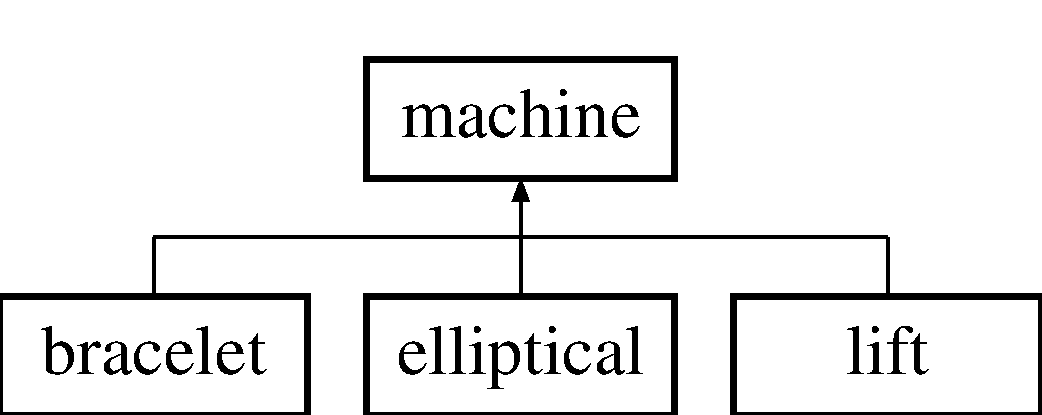
\includegraphics[height=2.000000cm]{classmachine}
\end{center}
\end{figure}
\subsection*{Public Member Functions}
\begin{DoxyCompactItemize}
\item 
\hypertarget{classmachine_a98793c9fe9044a6e6c12ded0ac96fcea}{{\bfseries machine} (std\-::string)}\label{classmachine_a98793c9fe9044a6e6c12ded0ac96fcea}

\item 
\hypertarget{classmachine_afb003d4605d7caec368eed19d73bb510}{std\-::string {\bfseries get\-\_\-name} () const }\label{classmachine_afb003d4605d7caec368eed19d73bb510}

\item 
\hypertarget{classmachine_a867d5d161df0799c6c4c3f5a39b594da}{void {\bfseries set\-\_\-name} (std\-::string)}\label{classmachine_a867d5d161df0799c6c4c3f5a39b594da}

\item 
\hypertarget{classmachine_a16f102ccb934d03c6cf8c2fd01da4b89}{\hyperlink{classmachine}{machine} $\ast$ {\bfseries clone} ()}\label{classmachine_a16f102ccb934d03c6cf8c2fd01da4b89}

\end{DoxyCompactItemize}
\subsection*{Protected Attributes}
\begin{DoxyCompactItemize}
\item 
\hypertarget{classmachine_aef2de447421299179c1417856bb3caa7}{std\-::string {\bfseries machine\-\_\-name}}\label{classmachine_aef2de447421299179c1417856bb3caa7}

\item 
\hypertarget{classmachine_ac158712554f0089431527276b170ff39}{std\-::string {\bfseries machine\-\_\-type}}\label{classmachine_ac158712554f0089431527276b170ff39}

\end{DoxyCompactItemize}


The documentation for this class was generated from the following files\-:\begin{DoxyCompactItemize}
\item 
machine.\-h\item 
machine.\-cpp\end{DoxyCompactItemize}

\hypertarget{classmachines_1_1Machines}{\section{machines\-:\-:Machines Class Reference}
\label{classmachines_1_1Machines}\index{machines\-::\-Machines@{machines\-::\-Machines}}
}
Inheritance diagram for machines\-:\-:Machines\-:\begin{figure}[H]
\begin{center}
\leavevmode
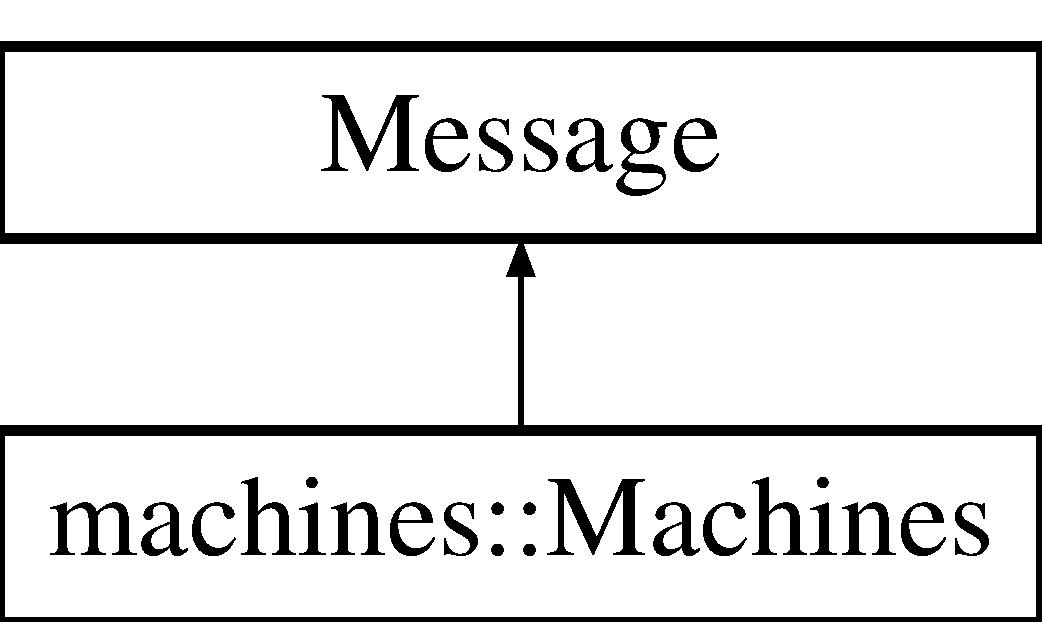
\includegraphics[height=2.000000cm]{classmachines_1_1Machines}
\end{center}
\end{figure}
\subsection*{Public Member Functions}
\begin{DoxyCompactItemize}
\item 
\hypertarget{classmachines_1_1Machines_a292be0e091155d3e56f6bcb4c6fe4016}{{\bfseries Machines} (const \hyperlink{classmachines_1_1Machines}{Machines} \&from)}\label{classmachines_1_1Machines_a292be0e091155d3e56f6bcb4c6fe4016}

\item 
\hypertarget{classmachines_1_1Machines_a965e237f4abb844d6c92a739580a856e}{\hyperlink{classmachines_1_1Machines}{Machines} \& {\bfseries operator=} (const \hyperlink{classmachines_1_1Machines}{Machines} \&from)}\label{classmachines_1_1Machines_a965e237f4abb844d6c92a739580a856e}

\item 
\hypertarget{classmachines_1_1Machines_a2cc3a0c6010471ca3cc9e9ef3cfc03d2}{const \\*
\-::google\-::protobuf\-::\-Unknown\-Field\-Set \& {\bfseries unknown\-\_\-fields} () const }\label{classmachines_1_1Machines_a2cc3a0c6010471ca3cc9e9ef3cfc03d2}

\item 
\hypertarget{classmachines_1_1Machines_a1bb257541a8104e793979c6cb552b586}{inline\-::google\-::protobuf\-::\-Unknown\-Field\-Set $\ast$ {\bfseries mutable\-\_\-unknown\-\_\-fields} ()}\label{classmachines_1_1Machines_a1bb257541a8104e793979c6cb552b586}

\item 
\hypertarget{classmachines_1_1Machines_a1a3bc0fb33034e59799630e9e117340d}{void {\bfseries Swap} (\hyperlink{classmachines_1_1Machines}{Machines} $\ast$other)}\label{classmachines_1_1Machines_a1a3bc0fb33034e59799630e9e117340d}

\item 
\hypertarget{classmachines_1_1Machines_a9299e828801acf217451855f98dc3291}{\hyperlink{classmachines_1_1Machines}{Machines} $\ast$ {\bfseries New} () const }\label{classmachines_1_1Machines_a9299e828801acf217451855f98dc3291}

\item 
\hypertarget{classmachines_1_1Machines_ade18b2a1be4d42b8720d500235bbbb92}{\hyperlink{classmachines_1_1Machines}{Machines} $\ast$ {\bfseries New} (\-::google\-::protobuf\-::\-Arena $\ast$arena) const }\label{classmachines_1_1Machines_ade18b2a1be4d42b8720d500235bbbb92}

\item 
\hypertarget{classmachines_1_1Machines_a605afb96d88f75e6523709744accd994}{void {\bfseries Copy\-From} (const \-::google\-::protobuf\-::\-Message \&from)}\label{classmachines_1_1Machines_a605afb96d88f75e6523709744accd994}

\item 
\hypertarget{classmachines_1_1Machines_aa103bcd18a11a4ae4b5006c41a6963bd}{void {\bfseries Merge\-From} (const \-::google\-::protobuf\-::\-Message \&from)}\label{classmachines_1_1Machines_aa103bcd18a11a4ae4b5006c41a6963bd}

\item 
\hypertarget{classmachines_1_1Machines_a695a058ef121a3602a4a725986c23f1e}{void {\bfseries Copy\-From} (const \hyperlink{classmachines_1_1Machines}{Machines} \&from)}\label{classmachines_1_1Machines_a695a058ef121a3602a4a725986c23f1e}

\item 
\hypertarget{classmachines_1_1Machines_a47fe6f7006872d1259bdbaef151c6eff}{void {\bfseries Merge\-From} (const \hyperlink{classmachines_1_1Machines}{Machines} \&from)}\label{classmachines_1_1Machines_a47fe6f7006872d1259bdbaef151c6eff}

\item 
\hypertarget{classmachines_1_1Machines_a762a75918a2ab568b3900eadb63a2866}{void {\bfseries Clear} ()}\label{classmachines_1_1Machines_a762a75918a2ab568b3900eadb63a2866}

\item 
\hypertarget{classmachines_1_1Machines_a46c08283129db4b3994306b6a64ee623}{bool {\bfseries Is\-Initialized} () const }\label{classmachines_1_1Machines_a46c08283129db4b3994306b6a64ee623}

\item 
\hypertarget{classmachines_1_1Machines_a75b8614e34090cdf79e1992a40f6ea6c}{int {\bfseries Byte\-Size} () const }\label{classmachines_1_1Machines_a75b8614e34090cdf79e1992a40f6ea6c}

\item 
\hypertarget{classmachines_1_1Machines_ad36cc5fe851a9bb2353bdeda8992268e}{bool {\bfseries Merge\-Partial\-From\-Coded\-Stream} (\-::google\-::protobuf\-::io\-::\-Coded\-Input\-Stream $\ast$input)}\label{classmachines_1_1Machines_ad36cc5fe851a9bb2353bdeda8992268e}

\item 
\hypertarget{classmachines_1_1Machines_a0e9d435e3d34ca4f8f38193c80d594fb}{void {\bfseries Serialize\-With\-Cached\-Sizes} (\-::google\-::protobuf\-::io\-::\-Coded\-Output\-Stream $\ast$output) const }\label{classmachines_1_1Machines_a0e9d435e3d34ca4f8f38193c80d594fb}

\item 
\hypertarget{classmachines_1_1Machines_a099db6b410274cfbefa04a846a3cd878}{\-::google\-::protobuf\-::uint8 $\ast$ {\bfseries Serialize\-With\-Cached\-Sizes\-To\-Array} (\-::google\-::protobuf\-::uint8 $\ast$output) const }\label{classmachines_1_1Machines_a099db6b410274cfbefa04a846a3cd878}

\item 
\hypertarget{classmachines_1_1Machines_a34a4b4e07ff4b4533120ceace8a978f8}{int {\bfseries Get\-Cached\-Size} () const }\label{classmachines_1_1Machines_a34a4b4e07ff4b4533120ceace8a978f8}

\item 
\hypertarget{classmachines_1_1Machines_a9e3cb699d42495f73e09ef78bdedb2eb}{\-::google\-::protobuf\-::\-Metadata {\bfseries Get\-Metadata} () const }\label{classmachines_1_1Machines_a9e3cb699d42495f73e09ef78bdedb2eb}

\item 
\hypertarget{classmachines_1_1Machines_a61b3c3827f4473c4ae4dacb70de89b7e}{int {\bfseries machine\-\_\-size} () const }\label{classmachines_1_1Machines_a61b3c3827f4473c4ae4dacb70de89b7e}

\item 
\hypertarget{classmachines_1_1Machines_ae910dc1ade7da741cbf1d0585bae15e4}{void {\bfseries clear\-\_\-machine} ()}\label{classmachines_1_1Machines_ae910dc1ade7da741cbf1d0585bae15e4}

\item 
\hypertarget{classmachines_1_1Machines_aa8191eefb09e64b6b0b1014065582a81}{const \-::\hyperlink{classmachines_1_1Machine}{machines\-::\-Machine} \& {\bfseries machine} (int index) const }\label{classmachines_1_1Machines_aa8191eefb09e64b6b0b1014065582a81}

\item 
\hypertarget{classmachines_1_1Machines_a46d3142739a905e6b942d2b1524c7267}{\-::\hyperlink{classmachines_1_1Machine}{machines\-::\-Machine} $\ast$ {\bfseries mutable\-\_\-machine} (int index)}\label{classmachines_1_1Machines_a46d3142739a905e6b942d2b1524c7267}

\item 
\hypertarget{classmachines_1_1Machines_a7ee40fc6cbd46314c0532a8a635d79a2}{\-::\hyperlink{classmachines_1_1Machine}{machines\-::\-Machine} $\ast$ {\bfseries add\-\_\-machine} ()}\label{classmachines_1_1Machines_a7ee40fc6cbd46314c0532a8a635d79a2}

\item 
\hypertarget{classmachines_1_1Machines_a76d1b295f2268d52ea966f2812877df8}{\-::google\-::protobuf\-::\-Repeated\-Ptr\-Field\\*
$<$ \-::\hyperlink{classmachines_1_1Machine}{machines\-::\-Machine} $>$ $\ast$ {\bfseries mutable\-\_\-machine} ()}\label{classmachines_1_1Machines_a76d1b295f2268d52ea966f2812877df8}

\item 
\hypertarget{classmachines_1_1Machines_ad023d0f06d19351ecd167f54317c517c}{const \\*
\-::google\-::protobuf\-::\-Repeated\-Ptr\-Field\\*
$<$ \-::\hyperlink{classmachines_1_1Machine}{machines\-::\-Machine} $>$ \& {\bfseries machine} () const }\label{classmachines_1_1Machines_ad023d0f06d19351ecd167f54317c517c}

\end{DoxyCompactItemize}
\subsection*{Static Public Member Functions}
\begin{DoxyCompactItemize}
\item 
\hypertarget{classmachines_1_1Machines_a52bf81fa69df98a1678a0fa4348aa881}{static const \\*
\-::google\-::protobuf\-::\-Descriptor $\ast$ {\bfseries descriptor} ()}\label{classmachines_1_1Machines_a52bf81fa69df98a1678a0fa4348aa881}

\item 
\hypertarget{classmachines_1_1Machines_a8dd32d0d5d1c9eb75693426e1451a197}{static const \hyperlink{classmachines_1_1Machines}{Machines} \& {\bfseries default\-\_\-instance} ()}\label{classmachines_1_1Machines_a8dd32d0d5d1c9eb75693426e1451a197}

\end{DoxyCompactItemize}
\subsection*{Static Public Attributes}
\begin{DoxyCompactItemize}
\item 
\hypertarget{classmachines_1_1Machines_a005ddddbd827ea28365be296f13ca5e2}{static const int {\bfseries k\-Machine\-Field\-Number} = 1}\label{classmachines_1_1Machines_a005ddddbd827ea28365be296f13ca5e2}

\end{DoxyCompactItemize}
\subsection*{Friends}
\begin{DoxyCompactItemize}
\item 
\hypertarget{classmachines_1_1Machines_a8630324413f042411acb26cd21efd53e}{void {\bfseries protobuf\-\_\-\-Add\-Desc\-\_\-fitplanet\-\_\-2eproto} ()}\label{classmachines_1_1Machines_a8630324413f042411acb26cd21efd53e}

\item 
\hypertarget{classmachines_1_1Machines_a005300ae4e9313c5f2d6ed15f4f18d7f}{void {\bfseries protobuf\-\_\-\-Assign\-Desc\-\_\-fitplanet\-\_\-2eproto} ()}\label{classmachines_1_1Machines_a005300ae4e9313c5f2d6ed15f4f18d7f}

\item 
\hypertarget{classmachines_1_1Machines_a3942eb78a8614c8d9d4994d09c14849d}{void {\bfseries protobuf\-\_\-\-Shutdown\-File\-\_\-fitplanet\-\_\-2eproto} ()}\label{classmachines_1_1Machines_a3942eb78a8614c8d9d4994d09c14849d}

\end{DoxyCompactItemize}


The documentation for this class was generated from the following files\-:\begin{DoxyCompactItemize}
\item 
fitplanet.\-pb.\-h\item 
fitplanet.\-pb.\-cc\end{DoxyCompactItemize}

\hypertarget{classmember}{\section{member Class Reference}
\label{classmember}\index{member@{member}}
}
Inheritance diagram for member\-:\begin{figure}[H]
\begin{center}
\leavevmode
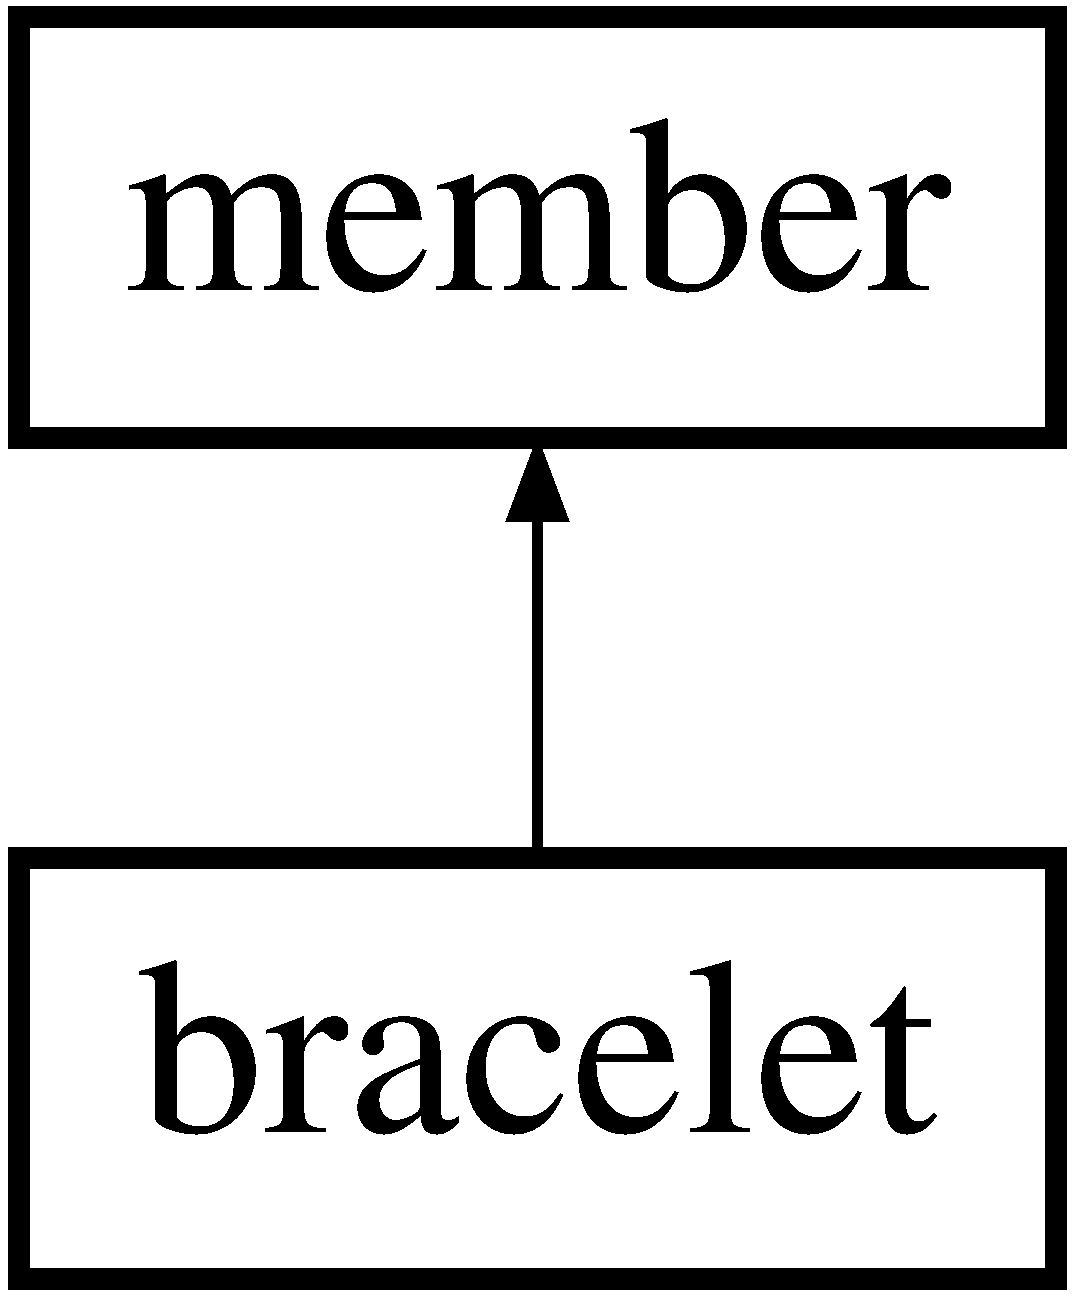
\includegraphics[height=2.000000cm]{classmember}
\end{center}
\end{figure}
\subsection*{Public Member Functions}
\begin{DoxyCompactItemize}
\item 
\hypertarget{classmember_a209a0e52f9163bfc398c5fb1dd990d61}{{\bfseries member} (char $\ast$, int)}\label{classmember_a209a0e52f9163bfc398c5fb1dd990d61}

\item 
\hypertarget{classmember_ae822170dd36d4e8733695ec2dabdeb33}{char $\ast$ {\bfseries get\-\_\-name} () const }\label{classmember_ae822170dd36d4e8733695ec2dabdeb33}

\item 
\hypertarget{classmember_a5e2b9da294c4c309d006e381ae459aa7}{int {\bfseries get\-\_\-contract} () const }\label{classmember_a5e2b9da294c4c309d006e381ae459aa7}

\item 
\hypertarget{classmember_ae9bc91157132af448c73d32fa69eaf71}{void {\bfseries set\-\_\-name} (char $\ast$)}\label{classmember_ae9bc91157132af448c73d32fa69eaf71}

\item 
\hypertarget{classmember_adf19ec5d197a949789ea2602b0e60849}{void {\bfseries renew\-\_\-contract} (int)}\label{classmember_adf19ec5d197a949789ea2602b0e60849}

\end{DoxyCompactItemize}


The documentation for this class was generated from the following files\-:\begin{DoxyCompactItemize}
\item 
member.\-h\item 
member.\-cpp\end{DoxyCompactItemize}

\hypertarget{structmachines_1_1StaticDescriptorInitializer__fitplanet__2eproto}{\section{machines\-:\-:Static\-Descriptor\-Initializer\-\_\-fitplanet\-\_\-2eproto Struct Reference}
\label{structmachines_1_1StaticDescriptorInitializer__fitplanet__2eproto}\index{machines\-::\-Static\-Descriptor\-Initializer\-\_\-fitplanet\-\_\-2eproto@{machines\-::\-Static\-Descriptor\-Initializer\-\_\-fitplanet\-\_\-2eproto}}
}


The documentation for this struct was generated from the following file\-:\begin{DoxyCompactItemize}
\item 
fitplanet.\-pb.\-cc\end{DoxyCompactItemize}

%--- End generated contents ---

% Index
\newpage
\phantomsection
\addcontentsline{toc}{chapter}{Index}
\printindex

\end{document}
